\label{voronoi}

In this chapter, we develop a novel analytic expression for the pursuit-evasion Voronoi diagram \cite{pachter2014active} that marks or borders the "safe" or "escape" region $R_{e}$ for the Target, i.e., the region defined by the set of all coordinate points $(x,y)$ such that if the target's initial position $(x_{T},y_{T})$ is inside this region, then the target is guaranteed to survive (to escape the Attacker) provided both the Target and Defender implement their optimal strategies, and regardless of the policy adopted by the Attacker, whether optimal or not.
The Voronoi diagram obtaind divides the $XY-$plane, into two regions 
\begin{itemize}
\item a safe or escape region $R_{e}$ to which the Defender's initial position $\boldsymbol{D}$ belongs.
\item a \textit{potentially} unsafe region to which the Attacker's initial position $\boldsymbol{A}$ belongs.
\end{itemize}
Garcia et al. \cite{pachter2014active} treated this problem for $\gamma=1$ only using some involved arguments with inequalities developed from scratch, and without due reference to their earlier analysis concerning the critical speed ratio.\\


A very important \textit{insight} that markedly simplifies our work is to note that required Voronoi diagram is simply a rephrasing of the criticality equation (\ref{eq36in3}) for any value of $\gamma$ including the cases $\gamma>1$ or $\gamma<1$ and $\gamma=1$, viewed as a relation between $y_{T}$ and $x_{T}$ rather than a polynomial in $\alpha$. Working with equalities is definitely simpler than working with inequalities, and it specifies a Voronoi diagram that divides the whole plane into two distinct parts, namely: the safe region and the (potentially) unsafe region. The safe region is then identified simply as the region to which $\boldsymbol{D}$ belongs. Note that the set of points of the safe regions $R_{e}$ is a superset of the points reachable by the Defender before the Attacker $R_{r}$, i.e., $R_{e}\supseteq R_{r}$. The two regions $R_{e}$ and $R_{r}$ are identical if the Target does not move at all ($\alpha=0$), a situation in which the Target does not exert any own effort to secure its survival and relies solely on the Defender's helping efforts. The family of Voronoi diagrams for various values of the normalized speed $\alpha$ will be bounded by the one for $\alpha=0$, which is the border of $R_r$ (Fig. \ref{Rr2}).\\
Now, we obtain the general Voronoi diagram by rewriting the critically equation (\ref{eq36in3}) or (\ref{generaleq4}) as a relation between $y_{T}$ and $x_{T}$. This is achieved via (\ref{d}) to substitute $(x_{A}^{2}+x_{T}^{2}-2x_{A}x_{T}+y_{T}^{2})$ for $d^{2}$. To avoid mistakes in the manipulations, one must make sure that the pertinent equation at every step is dimensionally homogeneous. From (\ref{generaleq4}), we write
\begin{equation}
(4\gamma \alpha x_{A})d= -(1-\gamma^{2})d^{2}
+4 \gamma^{2} x_{A} x_{T}
-4 \gamma^{2} \alpha^{2} x_{A}^{2}
\label{cr-eq-Vd}
\end{equation}

Now, we square both sides of (\ref{cr-eq-Vd}) to obtain

\begin{equation}
\begin{split}
16 \gamma^{2} \alpha^{2} x_{A}^{2} (x_{A}^{2} +x_{T}^{2}-2x_{A}x_{T}+y_{T}^{2})
&=[-(1-\gamma^{2})(x_{A}^{2} +x_{T}^{2}-2x_{A}x_{T}+y_{T}^{2})+4 \gamma^{2} x_{A} x_{T}-4 \gamma^{2} \alpha^{2} x_{A}^{2}]^{2}\\
&=[-(1-\gamma^{2})(x_{A}^{2}+x_{T}^{2}+y_{T}^{2})+2(1+\gamma^{2})x_{A}x_{T}-4 \gamma^{2} \alpha^{2} x_{A}^{2}]^{2}
\end{split}
\label{poly1}
\end{equation}

Now we rearrange (\ref{poly1}) as a quartic equation (forth-degree polynomial) in $x_{T}$ and $y_{T}$, namely

\begin{equation}
\begin{split}
p(x_T,y_T)& = 16 \gamma^2 \alpha^2 x_A^4 \\
          &+ 16 \gamma^2 \alpha^2 x_A^2 x_T^2\\
          &- 32 \gamma^2 \alpha^2 x_A^3 x_T \\
          &+ 16 \gamma^2 \alpha^2 x_A^2 y_T^2 \\
          &- (1-\gamma^2)^2 [x_A^4 + x_T^4 + y_T^4 + 2 x_A^2 x_T^2 
          + 2 x_A^2 y_T^2  +  2 x_T^2 y_T^2 ] \\
          &- (1 + \gamma^2)^2 * 4 x_A^2 x_T^2 \\ 
          &- 16 \gamma^4 \alpha^4 x_A^4 \\
          &+ 2 (1 - \gamma^4) (2 x_A^3 x_T + 2 x_A x_T^3 + 2 x_A x_T y_T^2) \\ 
          &- 8 \gamma^2 (1 - \gamma^2) \alpha^2 (x_A^4 + x_A^2 x_T^2 + x_A^2 y_T^2) \\
          &+ 16 \gamma^2 (1 + \gamma^2) \alpha^2 x_A^3 x_T
          \end{split}
          \label{poly2}
\end{equation}

Equation (\ref{poly2}) is satisfied by the required Voronoi diagram. The quartic polynomial $p(x_t,y_T)$ satisfies
\begin{equation}
p(x_T,-y_T)=p(x_T,y_T),
\end{equation}
since it has even powers only for $y_T$. This means $p(x_T,y_T)$ is an even function in $y_T$ and its graph in the $x_T-y_T$ plane is \textit{symmetric} w.r.t. the $x_T$-axis.

Though (\ref{poly2}) is a quartic equation, the actual Voronoi diagram is expected to be a quadratic curve and not a quartic curve.
Note that we performed a squaring operation in obtaining (\ref{generaleq4}) and hence for obtaining (\ref{poly2}), which doubled the pertinent degree from two to four. Hence, the Voronoi diagram is just a second-degree factor, part or branch of the fourth-degree curve depicted by (\ref{poly2}). We will be able to identify the correct Voronoi diagram by rejecting any part of the curve that lies in $R_{r}$, i.e., the correct Voronoi diagram should define the border of $R_{e}$ such that $R_{e}\supseteq R_{r}$.\\


Note that (\ref{poly2}) is the general equation for the Voronoi diagram in our current $TAD$ problem and it appears here for the first time. As a check on its correctness, we use it to produce the correct curve for $\gamma=1$, earlier obtained by Garcia et al. \cite{garcia2015escape}, namely
 
\begin{equation}
16 x_{A}^{2}[-(1-\alpha^{2})x_{T}^{2}+\alpha^{2} y_{T}^{2}]
=-16 x_{A}^{4}\alpha^2 (1-\alpha^{2}),
\label{poly2in3}
\end{equation}

or equivalently
\begin{equation}
\dfrac{x_{T}^{2}}{\alpha^{2}x_{A}^{2}}
- \dfrac{y_{T}^{2}}{(1-\alpha^{2})x_{A}^{2}}=1.
\label{hyperbola}
\end{equation}

Equation (\ref{poly2in3}) represents a hyperbola which is an open curve of two branches. Interestingly enough the term hyperbola is believed  to have been coined by our old friend Apollonius of Perga in his work on conic sections. This hyperbola is represented in Fig. \ref{hyperbola graph} and has the following properties:

\begin{itemize}
\item The hyperbola has two focal points $\boldsymbol{F_1}=(c,0)$ and $\boldsymbol{F_2}=(-c,0)$, where 
\begin{equation}
c^2= \alpha^2 x_A^2 + (1-\alpha^2)x_A^2=x_A^2,
\end{equation}
i.e. the focal points coincide with the initial positions of the Attacker $\boldsymbol{A}=(x_A,0)$ and the Defender $\boldsymbol{D}=(-x_A,0).$ Note that these two focal points are shared by an infinite set of curves for various values of $\alpha\ (0<\alpha<1)$. 
\item The line joining the  focal points, i.e., the \textit{transverse axis} coincides with the $x_T$-axis. The midpoint of the two focal points, i.e., the \textit{center} of the hyperbola, is the origin (0,0). The conjugate axis (the line perpendicular to the hyperbola's transverse axis through its center) is the $y_T$-axis.
\item The eccentricity of the hyperbola $e$ is
\begin{equation}
e=\dfrac{c}{\alpha x_A}=\dfrac{1}{\alpha}>1,
\end{equation}
where the fact that $e>1$ distinguishes the hyperbola from other conic sections, namely the ellipse (of $e<1$) and the parabola (of $e=1$). Note that the eccentricity $e$ equals the ratio of the distance $PF_i$ from a point $P$ on the hyperbola to one focus $F_i$ to the distance of the point to the corresponding directrix $PQ_i$, i.e.
\begin{equation}
PF_i = e\ PQ_i , \ \ \ i=1,2,
\end{equation}
\item The vertices of the hyperbola (its intersections with the $x_T$-axis) are at $(\alpha x_A,0)$ and $(-\alpha x_A,0)$, and hence approach the two focal points as $\alpha$ tends to 1 (from below).
\item Perpendicular to the transverse axis are the two directrices $D_1$ and $D_2$ given by
\begin{equation}
x_T = \mp \dfrac{\alpha x_A}{e} = \mp \alpha^2 x_A
\end{equation}
These directrices also approach the focal points when $\alpha\to1$.
\item The hyperbola has two asymptotes that intersect at its center, and are given by
\begin{equation}
y_T= \mp (\dfrac{\sqrt{1-\alpha^2}}{\alpha})x_T.
\end{equation}
For $0<\alpha<1$, the magnitude of the slope for an asymptote increases as $\alpha$ decreases and vice verse. Unlike the vertices and directrices, the asymptotes are independent of $x_A$.
\item As a special case of the polynomial $p(x_T,y_T)$, in (\ref{poly2}) the hyperbola (\ref{hyperbola}) is an even function of $y_T$ and hence is symmetric about the $x_T$-axis, Incidently the hyperbola is also even in $x_T$ and hence its two branches are symmetric about the $y_T$-axis but this observation is irrelevant since only one branch is retained in further study.
\item In the limit $(\alpha\to0)$, the hyperbola (\ref{hyperbola}) degenerates into the $y_T$-axis.
\item In the limit $(\alpha\to1)$, the right branch or the hyperbole (\ref{hyperbola}) degenerates into a ray emanating from $\boldsymbol{A}$ in the positive direction of the $x_T$-axis, while its left branch degenerates into a ray emanating from $\boldsymbol{D}$ in the opposite direction.
\end{itemize}    


\begin{figure}[htb]
\centering
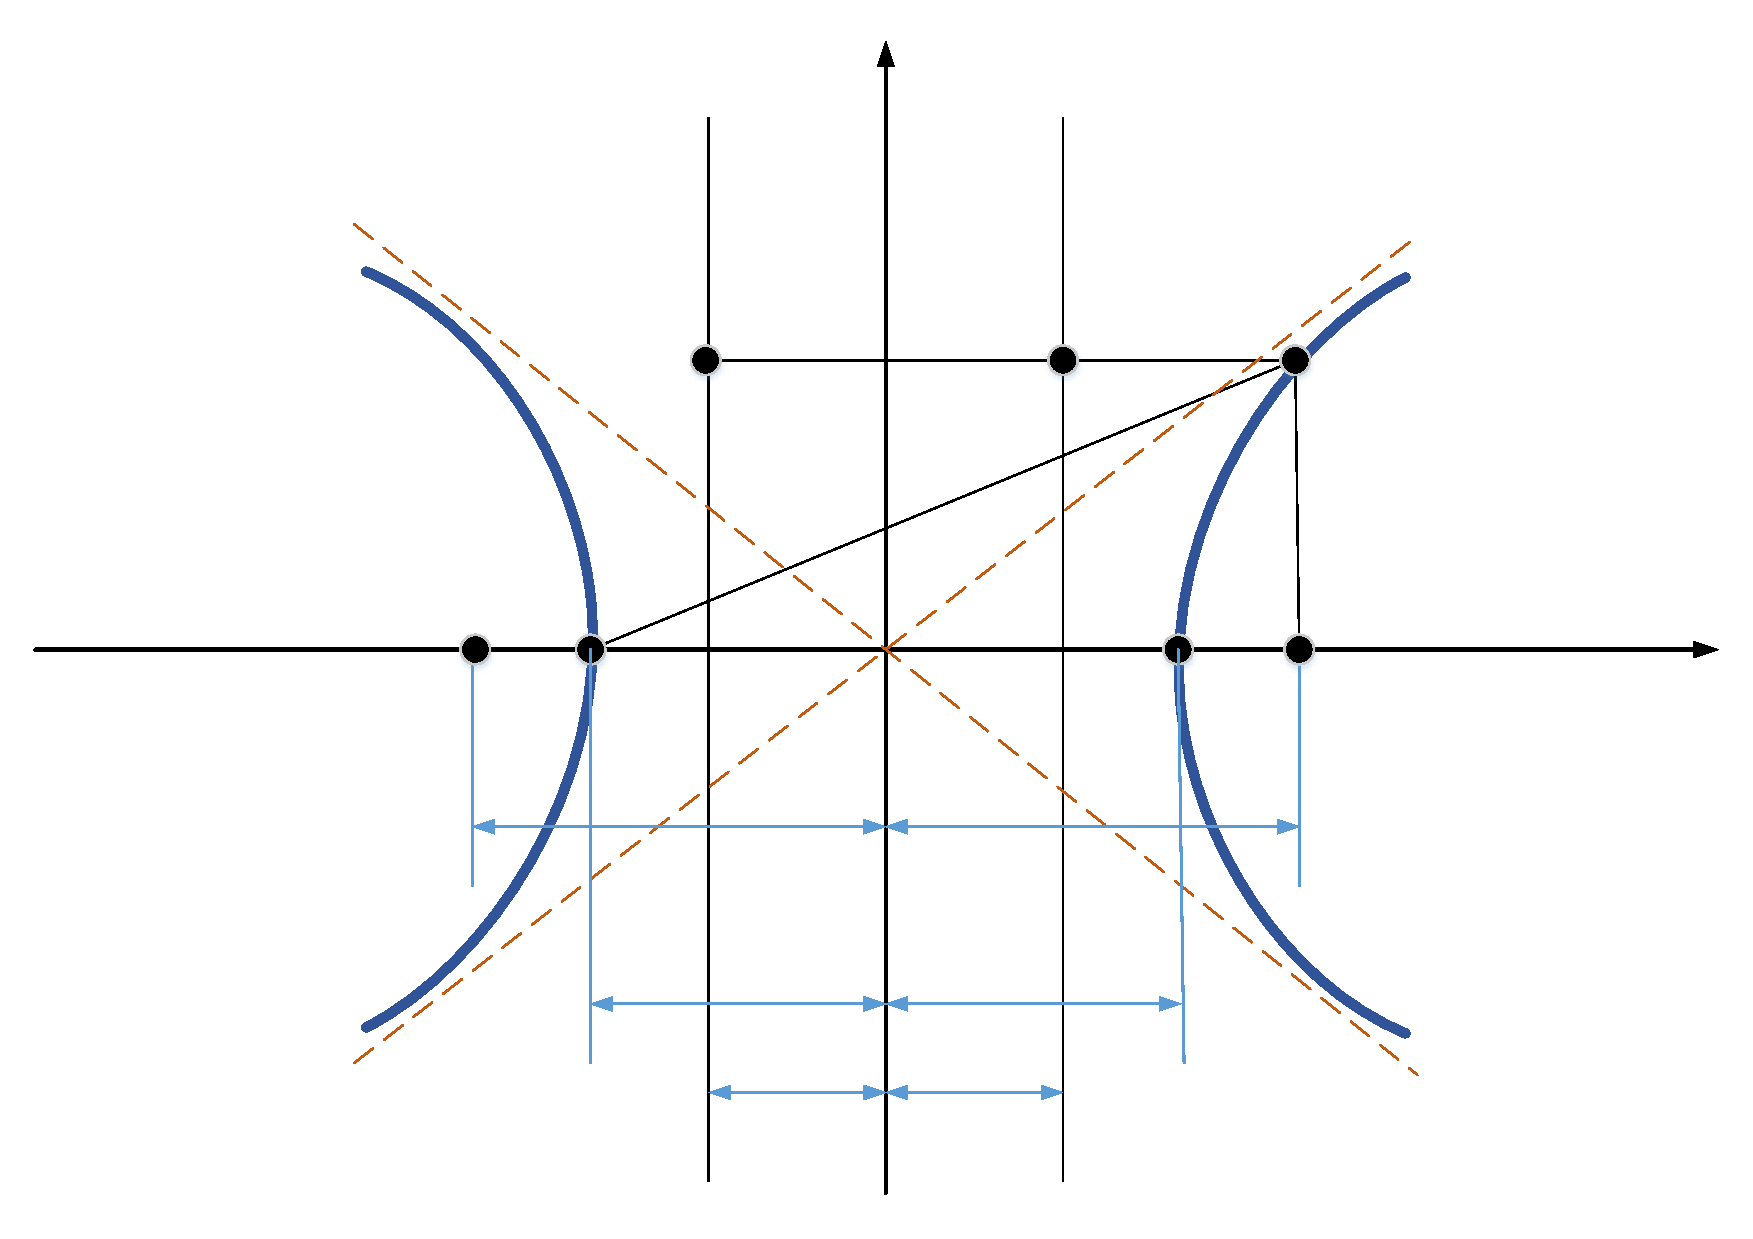
\includegraphics[width=0.95\textwidth]{fig/Drawing5_1.pdf}
\caption{Graph and features of the hyperbola $\dfrac{x_T^2}{\alpha^2 x_A^2} - \dfrac{y_T^2}{(1-\alpha^2)x_A^2}=1$ }
\label{hyperbola graph}
\end{figure}


In passing, we note that though equation (\ref{hyperbola}) was obtained herein as the special case $(\gamma=1)$ of equation $(\ref{poly2})$, we have first obtained it by a rephrasing of the criticality condition (\ref{case3_SD}) which holds for $\gamma=1$.\\


Now we note that the left branch of the hyperbola lies entirely in $R_{r}$ and hence it is rejected. The right branch of the hyperbola is the required Voronoi diagram, and it is bordering the escape region $R_{e}$ which extends to its left. Clearly, it is an enlargement of the reachability region $R_{r}$. Likewise, we expect the escape region to be a subset of the $AD$ Apollonius circle in Fig. \ref{2_g<1} where $\gamma<1$, and to be a superset of this circle in Fig. \ref{2_g>1} where $\gamma>1$.   

Figure \ref{gamma=1} is a sketch of the hyperbola (\ref{hyperbola}) for $\alpha=0.25$. the figure stresses that the right branch of the hyperbola is accepted as a Voronoi diagram while the left branch is rejected as such. Figure 5.3 is computer generated Voronoi diagrams for $\gamma=1$ and $\alpha$ varying from 0 (the $y_T$-axis) to slightly less than 1 (the straight-line ray emanating from $\boldsymbol{A}$ and coinciding with the $x_T$-axis).

Now, we come to a novel and really important contribution of this thesis, where we visualize the escape regions in the case of a fast Defender and a slow Defender. Figure \ref{gamma=0.8} shows the $AD$-Apollonius circle for $\gamma=0.8$ and $x_A=4$ for which $\boldsymbol{I_1}=(0.444,0)$, $\boldsymbol{E_1}=(36,0)$, $\boldsymbol{O_1}=(18.22,0)$, and $r_1=17.78$. Imposed on this circle is the quartic curve given by (\ref{poly2}) which consists of two closed curves. There is one closed curve entirely outside the $AD$-Apollonius circle, i.e., entirely inside the Reachability region $R_r$ and hence is rejected. The other closed curve is entirely inside the $AD$-Apollonius circle, i.e., the reachability region $R_r$ and hence it is accepted as the Voronoi diagram. The escape region (safe region) is the \textit{unshaded} area in this figure. Figure 5.5 generalizes Fig. \ref{gamma=0.8} by demonstrating various accepted branches of the Voronoi diagram for $\gamma=0.8$ and $\alpha$ as s parameter ranging from 0 (the $AD$-Apollonius circle) to a value approaching 1 from below (a closed curve collapsing to one barely encircling point A). This means that as $\alpha$ increases from 0 to 1, the safe or escape region expands from the exterior of the $AD$-Apollonius circle to almost the whole $x_T-y_T$ plane (excluding point A).


Now, we discuss the strikingly similar or dual case of a slow Defender. Figure \ref{gamma=1.25} shows the $AD$-Apollonius circle for $\gamma=1.25$ and $x_A=4$ for which $\boldsymbol{I_1}=(-0.444,0)$, $\boldsymbol{E_1}=(-36,0)$, $\boldsymbol{O_1}=(-18.22,0)$, $r_1=17.78$. Imposed on this circle is the quartic curve given by (\ref{poly2}). Note that the whole graph in Fig. \ref{gamma=1.25} is a \textit{mirror image} of that in Fig. \ref{gamma=0.8}. The quartic curve again consists of two closed curves. There is one closed curve entirely inside the $AD$-Apollonius circle. i.e., entirely inside the Reachability region $R_r$ and hence is rejected. The other closed curve is entirely outside the $AD$-Apollonius circle, i.e., entirely outside the Reachability region $R_r$, and hence is accepted as the Voronoi diagram. The escape region (safe region) is the \textit{shaded} area in this figure. Figure 5.7 generalizes Fig. \ref{gamma=1.25} by demonstrating various accepted branches of the Voronoi diagram for $\gamma=1.25$ and $\alpha$ as a parameter ranging from 0 (the $AD$-Apollonius circle) to a value approaching 1 from below.\\ 
    

In passing, we discuss the situation of $\gamma=0$ (when the Target does not move at all). In this case the $TA$ circle collapse into a single point $\boldsymbol{T}$ and the critically condition (\ref{generaleq4}) reduces to 

\begin{equation}
(1-\alpha^{2})d^{2}= 4 \gamma^{2} x_{T} x_{A}
\end{equation}

which can readily be written as 
\begin{equation}
(x_T-(\dfrac{1+\gamma^2}{1-\gamma^2})x_A)^2+(y_T-0)^2
=(\dfrac{2\gamma x_{A}}{1-\gamma^{2}})^{2}
\end{equation}

an equation that can be identified as the equation of the $AD$ Apollonius circle in the $Y_T-X_T$ coordinates.
This circle serves as the Voronoi diagram for $\alpha=0$, a fact confirming our assertion that the escape region $R_e$ reduces to the reachability region $R_r$ when $\alpha=0$. Likewise, when $\gamma=1$, imposing the condition $\alpha=0$ on the condition (\ref{case3_SD}) results in 
\begin{equation}
x_T=0
\end{equation} 
which means that the right branch of the hyperbolic Voronoi diagram (\ref{hyperbola}) degenerates into the $y_T-$axis (the perpendicular bisector of $\overline{AD}$) and again the region $R_e$ concides with the region $R_r$ in this case.


\begin{figure}[htb]
\centering
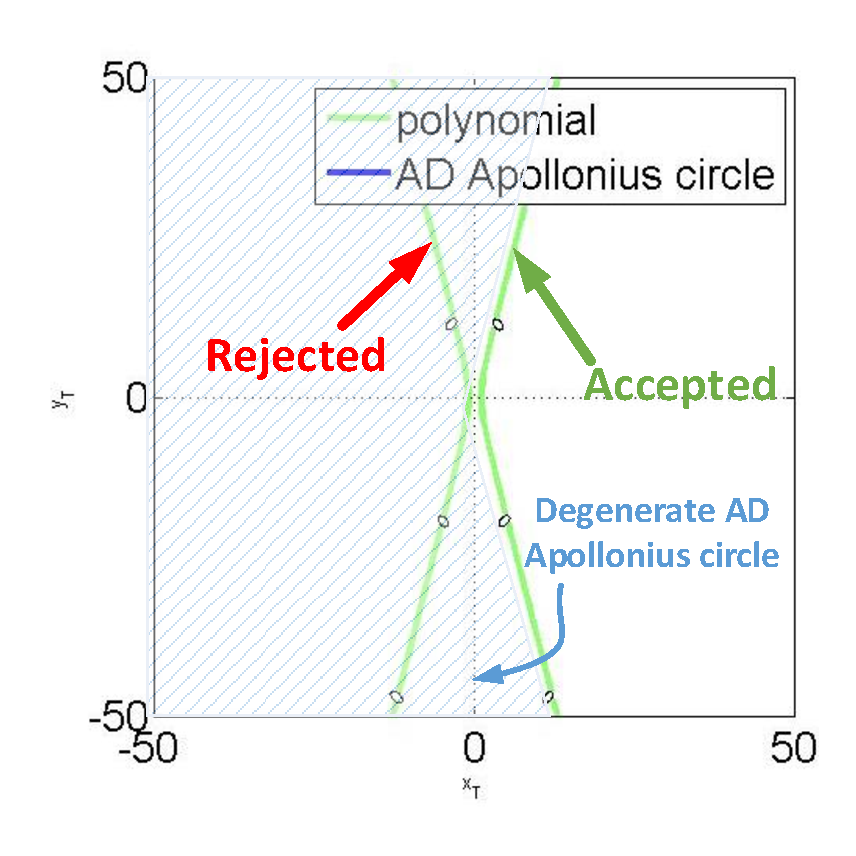
\includegraphics[width=0.66\textwidth]{fig/g_1.pdf}
\caption{Generated computer output for the Voronoi diagram bordering the safe region for $x_A=4,\ \alpha=0.25,\ \gamma=1$ (the safe region is the shaded area)}
\label{gamma=1}
\end{figure}

\begin{figure}[htb]
\centering
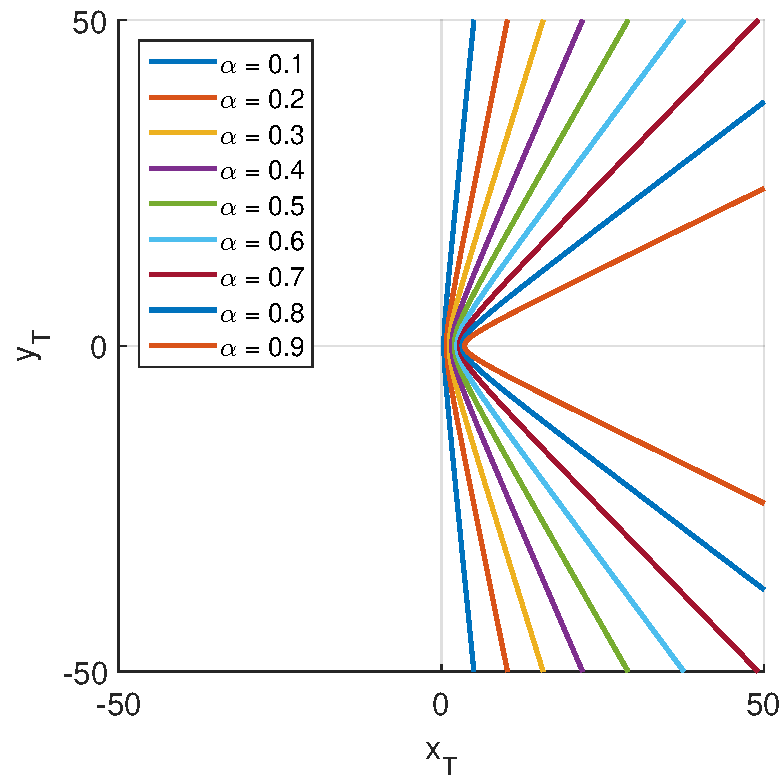
\includegraphics[width=0.66\textwidth]{fig/VAR_alpha_g_1.pdf}
\caption{Various accepted branches of the voronoi diagram for $\gamma=1$ and $\alpha$ as a parameter ranging from 0 to 1. These curves are computer generated from (\ref{poly2}) and (\ref{hyperbola})}
\label{VAR_alpha_gamma=1}
\end{figure}


\begin{figure}[htb]
\centering
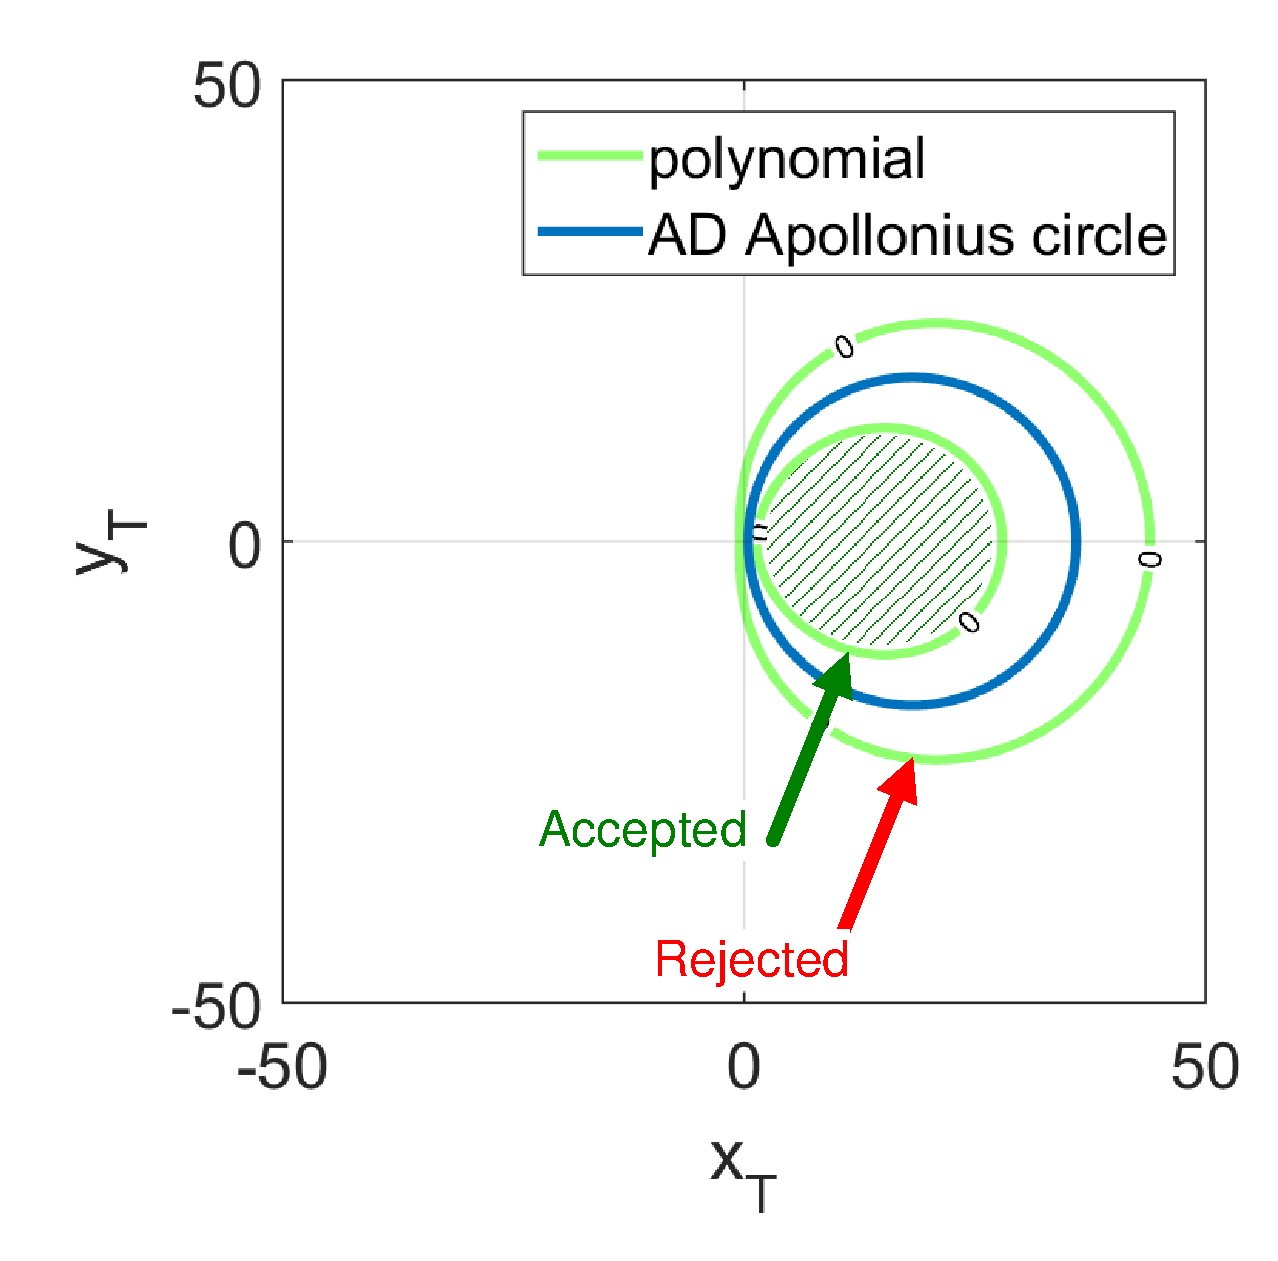
\includegraphics[width=0.66\textwidth]{fig/marked_circle_curve_g_0p8.pdf}
\caption{generated computer output for the Voronoi diagram bordering the safe region for $x_A=4,\ \alpha=0.25,\ \gamma=0.8$ (the safe region is the unshaded area) the quartic in (\ref{poly1}) or (\ref{poly2}) produces two closed curves: one outside the $AD$-Apollonius circle (rejected) and the other inside the circle (accepted as the Voronoi diagram)}
\label{gamma=0.8}
\end{figure}


\begin{figure}[htb]
\centering
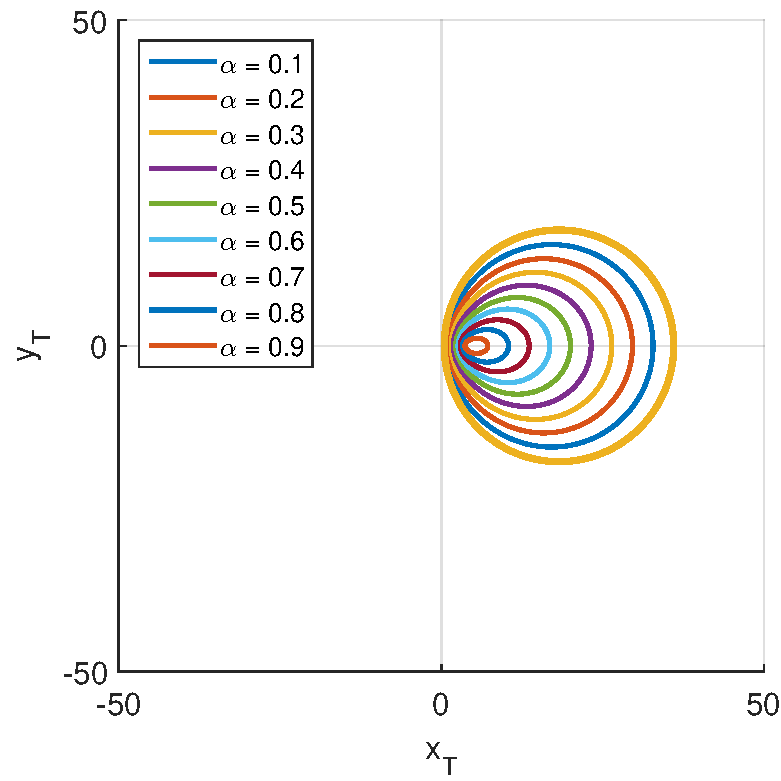
\includegraphics[width=0.66\textwidth]{fig/VAR_alpha_g_0p8.pdf}
\caption{Various accepted branches of the voronoi diagram for $\gamma=0.8$ and $\alpha$ as a parameter ranging from 0 to 1. These curves are computer generated from (\ref{poly2}) and (\ref{hyperbola})}
\label{VAR_alpha_gamma=0.8}
\end{figure}


\begin{figure}[htb]
\centering
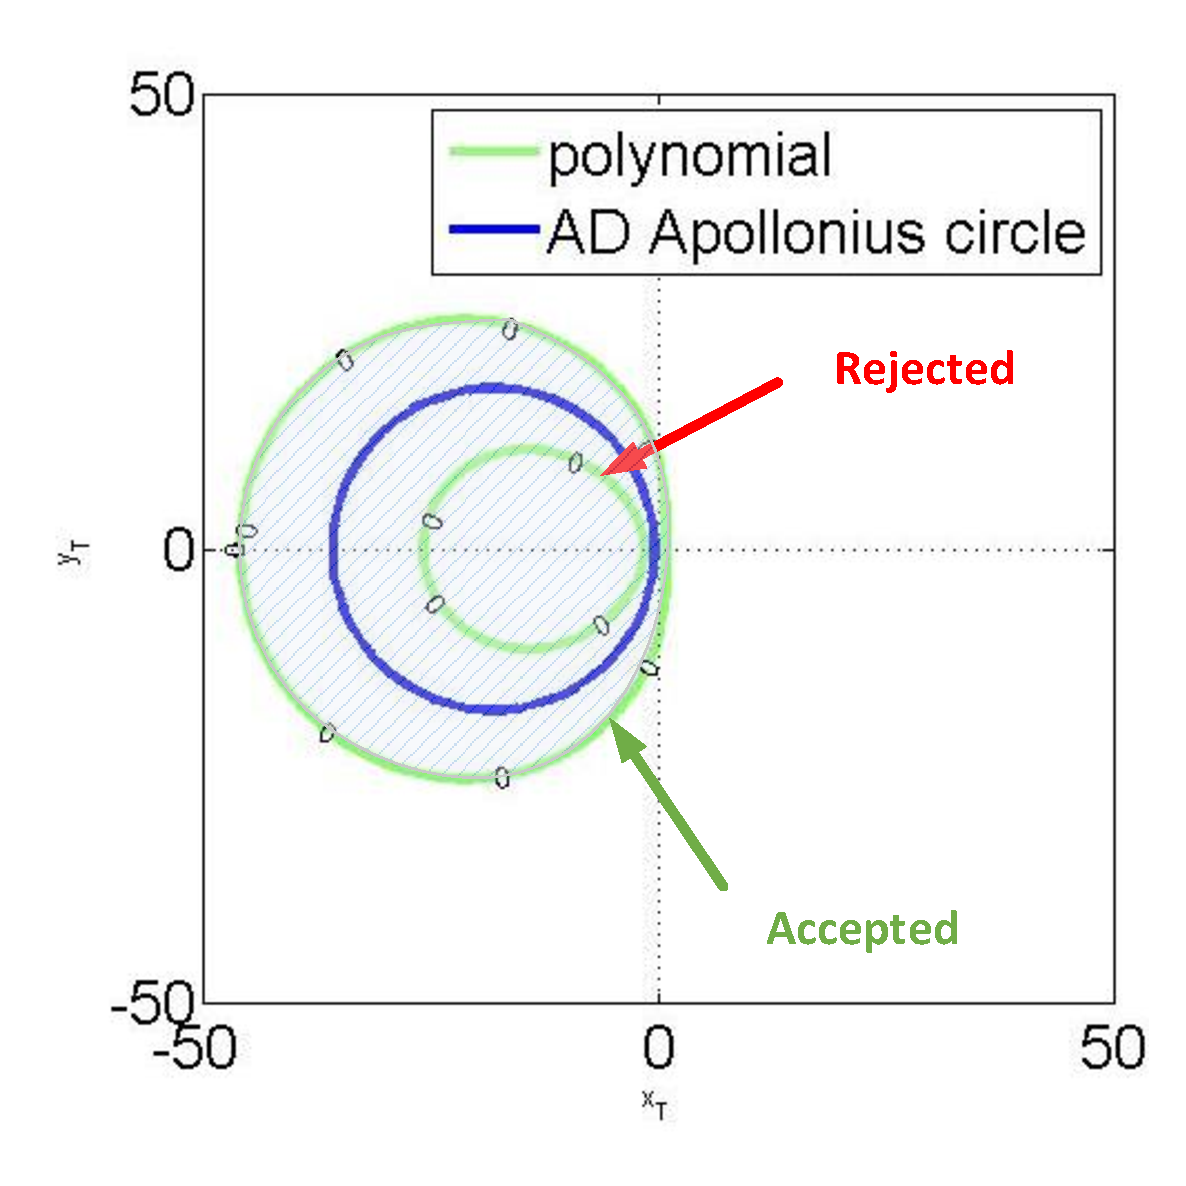
\includegraphics[width=0.66\textwidth]{fig/g_1p25.pdf}
\caption{generated computer output for the Voronoi diagram bordering the safe region for $x_A=4,\ \alpha=0.25,\ \gamma=1.25$ (the safe region is the shaded area) the quartic in (\ref{poly1}) or (\ref{poly2}) produces two closed curves: one inside the $AD$-Apollonius circle (rejected) and the other outside the circle (accepted as the Voronoi diagram)}
\label{gamma=1.25}
\end{figure}

\begin{figure}[htb]
\centering
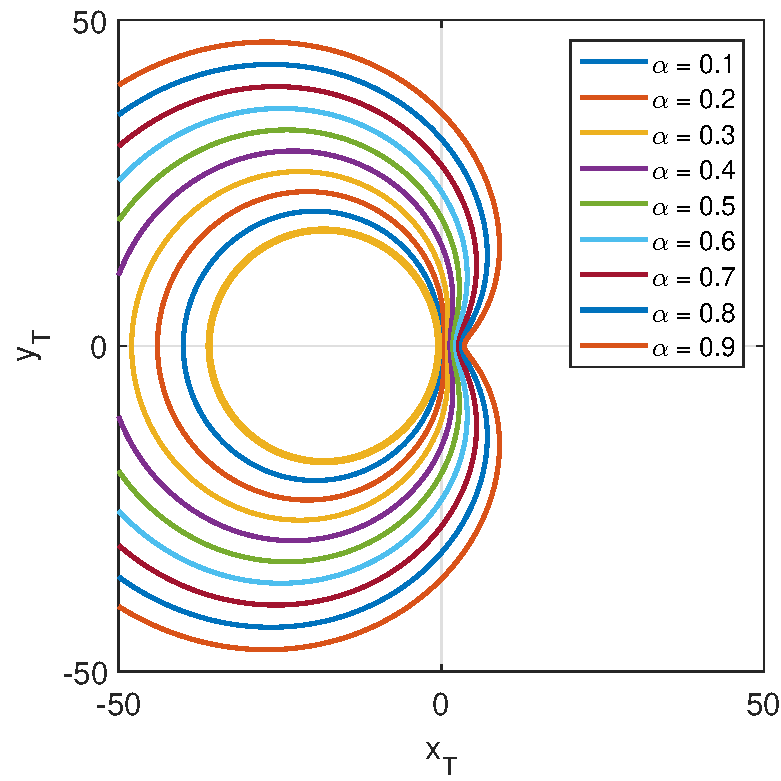
\includegraphics[width=0.66\textwidth]{fig/VAR_alpha_g_1p25.pdf}
\caption{Various accepted branches of the voronoi diagram for $\gamma=1.25$ and $\alpha$ as a parameter ranging from 0 to 1. These curves are computer generated from (\ref{poly2}) and (\ref{hyperbola})}
\label{VAR_alpha_gamma=1.25}
\end{figure}
